\documentclass[14pt]{extreport}
\usepackage[T1]{fontenc}
\usepackage[left=1in, right=1in, top=1in, bottom=1in]{geometry}
\usepackage{amsmath, amssymb, amsthm}
\usepackage{enumitem}
\usepackage{mathtools}
\usepackage{cancel}


\usepackage{bm}
% colored links
\usepackage{hyperref}
\hypersetup{
    colorlinks=true,
    linkcolor=blue,
    filecolor=magenta,      
    urlcolor=black!20!BurntOrange,
    }

% Inputting Python code
\usepackage[dvipsnames]{xcolor}
\definecolor{textblue}{rgb}{.2,.2,.7}
\definecolor{textred}{rgb}{0.54,0,0}
\definecolor{textgreen}{rgb}{0,0.43,0}
\usepackage{upquote}
\usepackage{listings}
\lstset{
    language=Python, 
    tabsize=4,
    basicstyle={\ttfamily},
    keywordstyle=\color{textblue},
    commentstyle=\color{textgreen},
    stringstyle=\color{textred},
    frame=none,
    columns=fullflexible,
    keepspaces=true,
    showstringspaces=false,
    xleftmargin=-15mm, % manual adjustment, figure out permanent solution
}

% Drawing figures
\usepackage{tikz}
\usetikzlibrary{matrix, positioning}
\usetikzlibrary{calc, shapes.symbols}

% Colored Boxes
\usepackage{tcolorbox}
\tcbuselibrary{skins,hooks}
\usetikzlibrary{shadows}
\usepackage{lipsum}

%Easy Numbering in case we add or remove questions
\newcounter{counter}
\newcommand{\Exercise}{Exercise \stepcounter{counter}\thecounter}

%Images
\usepackage{graphicx}
    \usepackage{subcaption}
    \usepackage{float}

%Formatting and Spacing
\setitemize[1]{noitemsep, parsep = 5pt, topsep = 5pt}
\setenumerate[1]{label = (\alph*), parsep = 1pt, topsep = 5pt}
\setlength\parindent{0pt}
\linespread{1.1}

%Cases Environment
\newlist{Cases}{enumerate}{3}
\setlist[Cases]{leftmargin = .25in, label = {Case \arabic*.}, topsep = 0.01in, itemsep = 0.04in, itemindent = .5in, parsep = 0in}

%Stats
\newcommand{\Cov}{\text{Cov}}
\newcommand{\trace}{\text{trace}}
\newcommand{\Normal}{\text{Normal}}
\newcommand{\var}[1]{\operatorname{var}\left(#1\right)}
\newcommand{\E}[2][]{\operatorname{E}_{#1}\left[#2\right]}
\renewcommand{\Pr}[2][]{\operatorname{P}_{#1}\left(#2\right)}


%Custom Title Fields
\newcommand{\lectTitle}{Exam 1 Review  Solutions}
\newcommand{\lectTime}{March 7, 2022}
\newcommand{\lectClass}{Advanced Algorithms}
\newcommand{\lectClassInstructor}{Dana Randall}
\newcommand{\lectSection}{Spring 2024}
\newcommand{\lectAuthorName}{Sarthak Mohanty}


\title{
    \vspace{1.75in}
    \textbf{\lectClass:\\ \lectTitle}\\
    \vspace{0.1in}\large{\textit{\lectClassInstructor\ \lectSection}}
    \vspace{2in}
    \author{\textbf{Sarthak Mohanty}}
    \date{}
}

\begin{document}

\maketitle
\pagebreak

\subsection*{\Exercise}
    A three-way cut is a set of edges such that removing it from the graph yields three connected components. Modify the min-cut algorithm discussed in class to get a three-way min cut. Compute the probability of success of your design and discuss how to boost it to be 1 - $o(1)$.

    \vspace{2mm}
    \textit{Hint: Stop looking stuff up, you don't need to! Use the process from class (taking special care near the end.)}


\subsection*{Solution}
    Let $G = (V, E)$ be a multigraph without self loops. For $e = (u, v) \in E$, define the contraction with respect to $e$ (denoted $G / e$) as in lecture. Now our algorithm is as follows:

    \vspace{2mm}
    Starting from the input graph $G = (V, E)$, repeat the following process until only \textit{four} vertices remain:
    \begin{enumerate}[label = \arabic*.]
        \item Choose an edge $e = (u, v)$ uniformly at random from $E$.
        \item Set $G = G / e$.
    \end{enumerate}
    Once four vertices remain, try all ways of partitioning these four vertices into three nonempty parts, and return the minimum three-way cut among them.

    \vspace{2mm}
    \textbf{Claim: } Let $\delta^{*}(S)$ be a three-way cut of minimum size of the graph $G = (V, E)$ with $|\delta^{*}(S)| = k$. Then the probability that the algorithm above returns a minimum three-way cut is at least $\frac{1}{\binom{n}{4}}$.

    \begin{proof}
    Denote the edges we contract in the algorithm as $\{e_{1}, e_{2}, \dots, e_{n - 4}\}$. The algorithm succeeds if none of the contracted edges are in $\delta^{*}(S)$.

    \vspace{5mm}
    First note that for every intermediate multigraph, the sum of the degrees for any \textit{pair} of vertices is at least $k$, otherwise we have a three-way cut of size smaller than $k$ by disconnecting two singular vertices from the rest of the graph. Thus the sum of the degrees for all pairs together is at least $ k \times \binom{|V|}{2} $, so
    $$\begin{alignedat}{2}
        & \quad \sum_{v \in V} \deg(v) \times (|V|-1) &&\ge k \times \binom{|V|}{2}  \\
         \Rightarrow& \quad \sum_{v \in V} \deg(v) \times (|V|-1) &&\ge \frac{k|V|(|V|-1)}{2} \\
         \Rightarrow& \quad \sum_{v \in V} \deg(v) &&\ge \frac{k|V|}{2}.
    \end{alignedat}$$
    We have shown the sum of all the degrees for every vertex in the graph is at least $\frac{k|V|}{2}$. Hence every intermediate graph with $|V|$ vertices has at least $\frac{k|V|}{4}$ edges.

    \vspace{5mm}
    We can now compute the probability that none of our contracted edges are in $\delta^{*}(S)$. After $j$ contractions, the resulting multigraph $G_{j}$ contains $n - j$ vertices, so
    $$|E(G_j)| \ge \frac{k(n - j)}{4}.$$
    Since there are exactly $k$ edges in $\delta^{*}(S)$, the probability that the next edge is bad is at most
    $$\frac{k}{k(n - j)/4} = \frac{4}{n - j}.$$
    Therefore,
    $$\begin{aligned}
        \Pr{\text{success}}
        &= \Pr{ e_{1}, \dots, e_{n - 4} \notin \delta^{*}(S)} \\
        &= \prod_{j = 0}^{n - 5}\Pr{\ e_{j + 1} \notin \delta^{*}(S) \mid e_{1}, \dots, e_{j} \notin \delta^{*}(S)\ } \\
        &\ge \prod_{j = 0}^{n - 5}\left(1 - \frac{4}{n - j}\right) \\
        &= \frac{n - 4}{n} \times \frac{n - 5}{n - 1} \times \frac{n - 6}{n - 2} \times \dots \times \frac{1}{5} \\
        &= \frac{4!}{n(n - 1)(n - 2)(n - 3)} \\
        &= \frac{1}{\binom{n}{4}}.
    \end{aligned}$$

    Now suppose no edge of $\delta^{*}(S)$ was contracted. Then the four remaining vertices still refine the original three parts of the optimal three-way cut. Therefore, among the constant number of three-way partitions of these four vertices, one of them corresponds exactly to $\delta^{*}(S)$. Since we explicitly try all of them and return the minimum, we return a minimum three-way cut.
    \end{proof}

    In order to boost the probability of success, we run the algorithm $c(n)\binom{n}{4}$ times, where $c(n) = \omega(1)$. Then the probability that at least one run succeeds is
    $$1 - \left(1 - \frac{1}{\binom{n}{4}}\right)^{c(n)\binom{n}{4}} \ge 1 - e^{-c(n)} = 1 - o(1).$$

    For example, running the algorithm $\binom{n}{4}\ln n$ times gives success probability at least
    $$1 - \frac{1}{n}.$$


\subsection*{\Exercise}
    \textit{(Navigating The Labyrinth)}
    The young maiden Ariadne is at the entrance of a simple labyrinth which branches in $m \ge 2$ corridors, as shown below. Unfortunately, she does not have her magic string with her! She knows the architect of the labyrinth, Daedalus, is somewhere in the labyrinth. She devises the following strategy to find him\footnote{This strategy is known as \textit{spiral search} and has been proven to be optimal. Looks like Ariadne was a Theory thread!}:

    \vspace{3mm}
    Continue until we reach $t$: execute cycles of steps, where the function determining the number of steps to walk before the $i$th turn starting from the origin is
    $$f(i) = \left(\frac{m}{m - 1}\right)^{i} \quad\forall i \ge 1$$
    What is the competitive ratio of this algorithm?

\begin{center}
    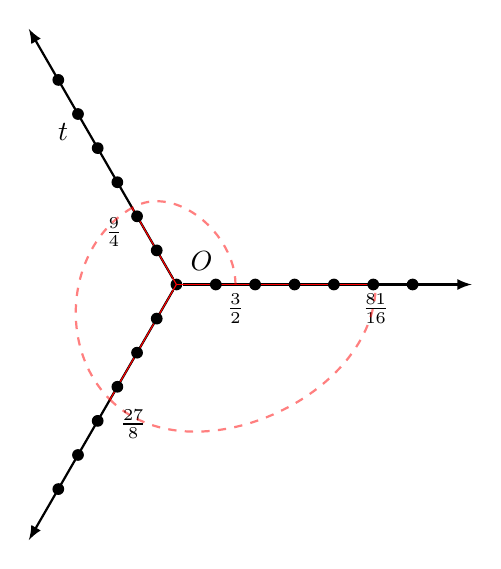
\begin{tikzpicture}[dot/.style={circle,fill,inner sep=1.5pt}, scale=0.5]
        \tikzset{>=latex}
        
        % Define the origin
        \node[dot,label=above right:$O$] (origin) at (0,0) {};
        
        % Calculate the ray length
        \pgfmathsetmacro{\raylength}{7.5}
        
        % Draw the rays at 120 degrees apart
        \foreach \a in {0,120,240} {
          \draw[thick,->] (origin) -- ++(\a:\raylength);
        }
        
        % Label
        \node at (120:5) [below left] {$t$};
        
        \node at (0:{3/2}) [below] {\small $\frac{3}{2}$};
        \node at (120:{9/4}) [below left] {\small $\frac{9}{4}$};
        \draw[red] (120:0) -- (120:{9/4});
        \node at (240:{27/8}) [below right] {\small $\frac{27}{8}$};
        \draw[red] (240:0) -- (240:{27/8});
        \node at (0:{81/16}) [below] {\small $\frac{81}{16}$};
        \draw[red] (0:0) -- (0:{81/16});
        
        % Spiral connection with dotted lines
        \draw[red, thick, dashed, opacity=0.5] (0:{3/2}) to [out=90,in=30] (120:{9/4});
        \draw[red, thick, dashed, opacity=0.5] (120:{9/4}) to [out=210,in=135] (240:{27/8});
        \draw[red, thick, dashed, opacity=0.5] (240:{27/8}) to [out=-45,in=270] (0:{81/16});
        
        
        % Place dots on the rays
        % R ray
        \foreach \r in {1,...,6} {
          \node[dot] at (\r,0) {};
          % t ray
          \node[dot] at (120:\r) {};
          % H ray
          \node[dot] at (240:\r) {};
        }
    \end{tikzpicture}
\end{center}

\subsection*{Solution}
    Let $r = \frac{m}{m - 1}$. Ariadne searches the $m$ corridors cyclically. If Daedalus is at distance $d$, the optimal offline cost is $OPT = d$.

    \vspace{2mm}
    Suppose Ariadne finds him on her $k$-th trip. Her total cost ($ALG$) includes the out-and-back walks for the first $k-1$ failed trips, plus the final one-way distance $d$:
    $$ALG = 2\sum_{i=1}^{k-1} r^i + d$$

    \vspace{2mm}
    To maximize the competitive ratio $ALG/OPT$, $d$ must be as small as possible. The worst case occurs when Daedalus is located infinitesimally beyond the distance Ariadne reached during her \textit{previous} visit to this exact same corridor. Because she cycles through $m$ corridors, her last visit to this corridor was $m$ steps ago. Thus, $d > r^{k-m}$. 

    \vspace{2mm}
    Using the geometric series bound $\sum_{i=1}^{k-1} r^i < \frac{r^k}{r-1}$, we bound the ratio:
    $$\frac{ALG}{OPT} = 1 + \frac{2\sum_{i=1}^{k-1} r^i}{d} < 1 + \frac{2 \left(\frac{r^k}{r-1}\right)}{r^{k-m}} = 1 + \frac{2r^m}{r-1}$$

    \vspace{2mm}
    Substituting $r = \frac{m}{m-1}$ (which implies $r-1 = \frac{1}{m-1}$), the competitive ratio evaluates to:
    $$1 + 2(m-1)\left(\frac{m}{m-1}\right)^m = 1 + \frac{2m^m}{(m-1)^{m-1}}.$$

\subsection*{\Exercise}
    \textit{(Potential Functions)} We discussed in class how potential functions were common motifs to help analyze online algorithms.
    
    \begin{enumerate}[label=(\alph*)]
        \item For an online algorithm $A$, let $c_A(\sigma)$ be the cost of the algorithm on the entire sequence and $c_A(i)$ be the cost on request $i$ (and similarly for $\text{OPT}$, the optimal offline algorithm). Prove the following. If for every request sequence $\sigma$ there exists a potential function $\Phi$ such that for all $1 \leq i \leq n$ we have
        $$c_A(i) + \Phi(i) - \Phi(i-1) \leq c \cdot c_{\text{OPT}}(i),$$ then $A$ is $c$-competitive.
        
        \item Consider the online problem \textsc{Read Into Buffer}: The task is to read an unknown-length non-empty string $s \in \Sigma^+$ of symbols into a buffer stored as contiguous array, one symbol at a time. The buffer must never be larger than $2|s|$ symbols. Reading a symbol has a basic cost of 1. When the currently allocated buffer is full, a new, larger array has to be allocated and the old contents must be copied, incurring a cost of 1 for each symbol already read. In other words, the cost for the $k$th symbol is either 1 (not full) or $k$ (full).
    
        \vspace{5mm}
        Devise an online algorithm for this problem and use a potential function to prove that its competitive ratio is at most 3.
    \end{enumerate}

\subsection*{Solution}
    \begin{enumerate}[label=(\alph*)]
        \item We assume the usual conditions that $\Phi(0) = 0$ and $\Phi(n) \ge 0$. Then summing over all requests gives
        $$
        \sum_{i = 1}^{n} c_A(i) + \sum_{i = 1}^{n} \left(\Phi(i) - \Phi(i - 1)\right) \le c \sum_{i = 1}^{n} c_{\text{OPT}}(i).
        $$
        The potential terms telescope, so
        $$
        c_A(\sigma) + \Phi(n) - \Phi(0) \le c \cdot c_{\text{OPT}}(\sigma).
        $$
        Since $\Phi(0) = 0$ and $\Phi(n) \ge 0$, we have
        $$
        c_A(\sigma) \le c_A(\sigma) + \Phi(n) \le c \cdot c_{\text{OPT}}(\sigma).
        $$
        Therefore $A$ is $c$-competitive.

        \item Use the natural doubling algorithm. Start with a buffer of size $1$. Whenever the buffer is full, allocate a new buffer of twice the size, copy over the old contents, and then insert the new symbol.

        \vspace{5mm}
        Let $n$ be the number of symbols currently stored and let $C$ be the current capacity. Define the potential function
        $$
        \Phi = 2n - C.
        $$
        After at least one symbol has been read, the doubling algorithm guarantees $n \le C < 2n$, so $\Phi \ge 0$.

        \vspace{5mm}
        There are two cases.

        \vspace{5mm}
        \textbf{Case 1: No resize occurs.} The actual cost is $1$. We increase $n$ by $1$, while $C$ stays fixed, so
        $$
        \Delta \Phi = 2.
        $$
        Thus the amortized cost is
        $$
        1 + 2 = 3.
        $$

        \textbf{Case 2: A resize occurs.} Suppose the old buffer is full, so $n = C$. We copy $C$ old symbols and insert the new one, so the actual cost is
        $$
        C + 1.
        $$
        Before resizing,
        $$
        \Phi_{\text{old}} = 2C - C = C.
        $$
        After resizing, the new capacity is $2C$ and the new number of stored symbols is $C + 1$, so
        $$
        \Phi_{\text{new}} = 2(C + 1) - 2C = 2.
        $$
        Therefore
        $$
        \Delta \Phi = 2 - C.
        $$
        So the amortized cost is
        $$
        (C + 1) + (2 - C) = 3.
        $$

        Thus every operation has amortized cost at most $3$. Since OPT has to pay at least $1$ per symbol, $\text{OPT} \ge |s|$. Therefore the doubling algorithm has competitive ratio at most $3$.
    \end{enumerate}

\subsection*{\Exercise}
    Define a preference list as \textit{cyclic} when it results in a cycle, for instance, where A prefers B over C, B prefers C over A, and C prefers A over B. Assess the accuracy of the following statement: A cyclic preference list leads to the existence of at least one stable marriage.

\subsection*{Solution}
    The statement is \textbf{not accurate as written}.

    \vspace{2mm}
    In the usual stable marriage problem, every person has a strict preference list over the people on the other side. In other words, each preference list is a total ordering. Under this assumption, a stable marriage always exists by the Gale-Shapley algorithm.

    \vspace{2mm}
    So the existence of a stable marriage does \textit{not} come from the preferences being cyclic. It comes from the fact that the preferences are complete strict rankings.

\subsection*{\Exercise}
    Consider a scenario in the stable marriage problem involving $n$ men and $n$ women. Determine the \textit{exact} maximum number of proposals that could occur when running the Gale-Shapely algorithm.

\subsection*{Solution}
    During the Gale-Shapley algorithm, a man never proposes to the same woman twice. Since there are $n$ men and $n$ women, there can be at most $n^{2}$ proposals total.

    \vspace{2mm}
    But we can do slightly better. The algorithm stops as soon as every man is matched. Therefore, the only way a man can propose to all $n$ women is if he is the last man to become matched. Every other man must be matched before proposing to all $n$ women, so each of the other $n - 1$ men proposes to at most $n - 1$ women.

    \vspace{2mm}
    Hence the total number of proposals is at most
    $$n + (n - 1)(n - 1).$$

    Simplifying,
    $$\begin{aligned}
        n + (n - 1)^2
        &= n + n^2 - 2n + 1 \\
        &= n^2 - n + 1.
    \end{aligned}$$

    Therefore, the number of proposals is at most
    $$n^{2} - n + 1.$$
    
    Now we show that this bound is achievable.

    \vspace{2mm}
    Let the men be $m_1, m_2, \dots, m_n$
    and the women be $w_1, w_2, \dots, w_n.$ Give every man the same preference list:
    $$w_1 \succ w_2 \succ \dots \succ w_n.$$

    Give the women preferences so that each of the first $n - 1$ women keeps rejecting the earlier men in favor of later men. For example,
    $$w_i: m_n \succ m_{n - 1} \succ \dots \succ m_1.$$

    Then the men fight over $w_1$, then over $w_2$, then over $w_3$, and so on. In the worst case, the algorithm forces all but one man to keep moving down their lists until only the last woman remains.

    \vspace{2mm}
    Thus the upper bound is tight, and the exact maximum number of proposals is
    $$n^{2} - n + 1.$$

\subsection*{\Exercise}
    Consider \textsc{FlushWhenFull} algorithm for paging: when a cache miss occurs and the entire cache is full, evict all pages from the cache. What is the competitive ratio of \textsc{FlushWhenFull}?

\subsection*{Solution}
    Obviously this is not a practical strategy. But, it turns out this has a competitive ratio of $k$. The proof is same as marking algorithm proof.
    
\subsection*{\Exercise}    
    Consider adding the power of limited lookahead to an algorithm for paging. Namely, fix a constant $f \in \mathbb{N}$. Upon receiving the current page $p_i$, the algorithm also learns $p_{i+1}, p_{i+2}, \dots, p_{i+f}$. Recall that the best achievable competitive ratio for deterministic algorithms without lookahead is $k$. Can you improve on this bound with lookahead?
    
\subsection*{Solution}
    An on-line algorithm does not gain any advantage in the worst case, since any request sequence $\sigma = \sigma_{1}, \dots, \sigma_{p}$ can be replaced by the request sequence $\sigma = (\sigma_{1})^{l}, \dots, (\sigma_{p})^{l}$ in which each request is repeated $l$ times, thus, hiding the future requests from the algorithm.

\subsection*{\Exercise}
    \textit{(Online Coloring)} We briefly covered coloring in our homework; now we will cover it in an online context. Our input sequence consists of the vertices $v_1, \ldots, v_n$ of an undirected graph $G = (\{v_1, \ldots, v_n\}, E)$. Together with each vertex $v_i$, we are given the list $E_i$ of all edges connecting $v_i$ to previously given vertices $v_1, \ldots, v_{i-1}$. Edges from $v_i$ to vertices $v_j$ with $j > i$ are only revealed once vertex $v_j$ is given. The number of edges and vertices in the graph is not known in advance.

    \vspace{5mm}
    When we are given $v_i$, we have to choose a color $c(v_i) \in \mathbb{N}$ for $v_i$ in such a way that no vertex adjacent to $v_i$ has color $c(v_i)$. As usual, this choice is final; we cannot change the color later on. We want to minimize the number of colors used.

    \vspace{5mm}
    We want to show that there is no deterministic $c$-competitive algorithm for this problem for any constant $c$. For any constant number $2 \leq k \in \mathbb{N}$ of colors and any deterministic online algorithm $A$, devise a strategy for an adversary that satisfies the following requirements.
    \begin{itemize}
      \item The strategy always produces a forest $T_{A,k}$.
      \item The online algorithm $A$ uses at least $k$ colors on $T_{A,k}$.
    \end{itemize}
    Offline, every forest can be colored with 2 colors; therefore, this implies that $A$'s competitive ratio is at least $k/2$.

\subsection*{Solution}
    We prove by induction that for any $k \geq 1$, an adversary can construct a forest forcing $A$ to use $k$ colors distributed across $k$ strictly distinct trees.

    \vspace{3mm}
    \textsc{Base Case} ($k=1$): The adversary reveals a single vertex. $A$ assigns it a color, trivially forming a forest with $1$ color in $1$ tree.

    \vspace{3mm}
    \textsc{Inductive Step}: Assume the claim holds for $k-1$. The adversary applies the $(k-1)$-strategy twice to generate two disjoint forests, $F_1$ and $F_2$. Let $C_1$ and $C_2$ be the sets of $k-1$ colors forced in each. By the hypothesis, the colored vertices in both forests lie in distinct trees.

    \vspace{2mm}
    If $C_1 \neq C_2$, then $|C_1 \cup C_2| \geq k$. The adversary stops. Since $F_1$ and $F_2$ are disjoint, we can trivially select $k$ distinct colors that lie in separate trees.

    \vspace{2mm}
    If $C_1 = C_2$, the adversary reveals a new vertex $x$. For each color in $C_1$, the adversary connects $x$ to the corresponding vertex in $F_1$. Because these vertices belong to disconnected trees in $F_1$, routing them through $x$ merges them into a single tree without creating cycles. 

    \vspace{2mm}
    Because $x$ borders every color in $C_1$, $A$ must assign $x$ a new color $c \notin C_1$. This single new tree containing $x$ (color $c$), alongside the $k-1$ unmodified trees in $F_2$ (colors $C_2 = C_1$), provides exactly $k$ colors across $k$ disjoint trees.

    \vspace{3mm}
    \textsc{Conclusion}: For any $k$, the adversary can force $A$ to use $k$ colors on a forest. Since forests are 2-colorable offline, $A$'s competitive ratio is at least $k/2$. Thus, no deterministic online algorithm is $c$-competitive for any constant $c$.

\subsection*{\Exercise\footnote{From Technische Universität Braunschweig.}}
    \textit{(Online Load Balancing)} We discussed load balancing quite a bit in the beginning of the semester. Here we consider a weighted variant. Suppose we receive a sequence of items, where $a_{i} \in (0, \infty)$ Moreover, we have a fixed number of $m$ bins with unlimited capacity. We have to pack each incoming item into a bin that we have to fix before the next item is given to us. As in load balancing, we want to minimize the total weight $W$ packed into the fullest bin.

    \vspace{5mm}
    We consider the following algorithm \textsc{GREEDY} for this problem. Initially, all bins are empty. On receiving the $i$th item $a_i$, \textsc{GREEDY} packs $a_i$ into the emptiest bin; ties are broken arbitrarily. For an example of the algorithm, refer to Figure 1.

\begin{figure}[H]
    \centering
    
\includegraphics[width=0.4\textwidth]{images/online_load_balancing_greedy.png}
    \caption{The packing that results from applying GREEDY to $m = 4$ bins and the input sequence $ (6, 7, 5, 11, 4, 5, 6) $. The quality of the solution produced by GREEDY is $W_G = 13$ (the fullest bin contains $7 + 6 = 13$ units of weight). The optimal solution has quality $W_O = 11$.}
    \label{fig:greedy_packing}
\end{figure}

\begin{enumerate}[label=(\arabic*)]
    \item Prove that \textsc{GREEDY} cannot be better than $ (2 - \frac{1}{m}) $-competitive. \textit{Hint: Consider a
    sequence that begins with small items and ends with a big item.}
    
    \item Prove that \textsc{GREEDY} is $ (2 - \frac{1}{m}) $-competitive. \textit{Hint: Consider the last item $a_T$ placed
    into the fullest bin and the value $W_G - a_T$.}
\end{enumerate}

\subsection*{Solution}
    Let $W_G$ be the maximum load produced by \textsc{GREEDY}, and $W_O$ be the optimal maximum load.

    \begin{enumerate}[label=(\arabic*)]
        \item Consider an input sequence of $m(m - 1)$ items of weight $1$, followed by a single item of weight $m$.

        \vspace{2mm}
        \textsc{GREEDY} perfectly balances the first $m(m - 1)$ items, placing exactly $m - 1$ items into each of the $m$ bins. The final item of weight $m$ is placed into any bin, yielding:
        $$W_G = (m - 1) + m = 2m - 1$$

        \vspace{2mm}
        The optimal solution isolates the weight-$m$ item in its own bin and distributes the $m(m - 1)$ small items equally among the remaining $m - 1$ bins (each also receiving a total load of $m$). Thus:
        $$W_O = m$$

        \vspace{2mm}
        This gives a competitive ratio of:
        $$\frac{W_G}{W_O} = \frac{2m - 1}{m} = 2 - \frac{1}{m}$$

        \item
        Let $a_T$ be the final item placed into the bin that ultimately reaches the maximum load $W_G$.

        \vspace{2mm}
        Because \textsc{GREEDY} assigns items to the emptiest bin, every other bin must have had a load of at least $W_G - a_T$ immediately prior to $a_T$'s placement. Therefore, the total weight of all items is at least $m(W_G - a_T) + a_T$.

        \vspace{2mm}
        The optimal solution distributes this same total weight across $m$ bins, meaning its maximum load must be at least the average:
        $$W_O \ge \frac{m(W_G - a_T) + a_T}{m} = W_G - a_T + \frac{a_T}{m}$$

        \vspace{2mm}
        Rearranging this inequality isolates $W_G$:
        $$W_G \le W_O + \left(1 - \frac{1}{m}\right)a_T$$

        \vspace{2mm}
        Since the optimal packing must accommodate $a_T$ in \textit{some} bin, it must be true that $W_O \ge a_T$. Substituting this bounds the ratio:
        $$W_G \le W_O + \left(1 - \frac{1}{m}\right)W_O = \left(2 - \frac{1}{m}\right)W_O$$

        \vspace{2mm}
        Thus, \textsc{GREEDY} is at most $(2 - \frac{1}{m})$-competitive.
    \end{enumerate}

\subsection*{\Exercise\footnote{Taken from CMU's 15-451/651 recitation.}}
    (\textit{k-wise Independent Hashing}) We can extend our definition of $k$-wise independence to hashing as well. A hash family $\mathcal{H}$ is \textit{k-wise independent} if for all $k$ distinct keys $x_1, x_2, \ldots, x_k \in \mathcal{U}$ and every set of $k$ values $v_1, v_2, \ldots, v_k \in \{0, 1, \ldots, m-1\}$, we have that $$ \Pr[h \in \mathcal{H}]{h(x_1) = v_1 \land h(x_2) = v_2 \land \ldots \land h(x_k) = v_k} = \frac{1}{m^k} $$
    Intuitively, this means that if you look at only up to $k$ keys, the hash family appears to hash them truly randomly.
    \begin{enumerate}
        \item Is this hash family from $U = \{a, b\}$ to $\{0, 1\}$ (i.e., $m = 2$) one-wise independent (i.e., uniform)? how about pairwise independent?
        
        $$\arraycolsep=7pt
        \begin{array}{c|cc}
        & a & b \\
        \hline
        h_1 & 0 & 0 \\
        h_2 & 1 & 0 \\
        \end{array}
        $$
        
        \item Can you fill in the blanks in this hash family with values in $\{0, 1\}$ to make it pairwise independent? 3-wise independent?
        
        $$\arraycolsep=7pt
        \begin{array}{c|ccc}
        & a & b & c \\
        \hline
        h_1 & 0 & 0 &  \\
        h_2 &  &  & 1 \\
        h_3 & 0 &  &  \\
        h_4 & 1 & 1 & 0 \\
        \end{array}
        $$
    \end{enumerate}

\subsection*{Solution}
    \begin{enumerate}
        \item 
        \begin{enumerate}[label=\roman*.]
            \item One-wise independence implies that for each key, each hash value in the range $ \{0, 1\} $ must occur with equal probability $ \frac{1}{2} $. But for key $b$, we have $ \Pr{h(b) = 0} = 1 $ (since both $ h_1(b) $ and $ h_2(b) $ are $ 0 $), so $\mathcal{H}$ is not one-wise independent.
            \item Pairwise independence requires that for any two distinct keys, the probability of them mapping to any two hash values is $\frac{1}{4}$. But for keys $ a, b $, we have $\Pr{h(a) = 0 \land h(b) = 1} = 0,$ so $\mathcal{H}$ is not pairwise independent.
        \end{enumerate}
        \item 
        \begin{enumerate}[label=\roman*.]
            \item For pairwise independence, each pair of distinct keys should map to any pair of values with equal probability $ \frac{1}{4} $. One possible solution is as follows:
            \[\arraycolsep=7pt
            \begin{array}{c|ccc}
                & a & b & c \\
                \hline
                h_1 & 0 & 0 & 0 \\
                h_2 & 1 & 0 & 1 \\
                h_3 & 0 & 1 & 1 \\
                h_4 & 1 & 1 & 0 \\
            \end{array}
            \]
            \item For 3-wise independence, each trio of distinct keys should map to any trio of values with equal probability $ \frac{1}{8} $. Achieving 3-wise independence requires 8 distinct hash functions for a range of $ \{0, 1\} $. With only 4 hash functions, we cannot achieve 3-wise independence for this hash family.
        \end{enumerate}
    
    \end{enumerate}

\section*{\Exercise}
    Here we consider a classic 2-universal hash function. Consider a universe where the keys are $k$ bits long, so $U = 0, \dots, 2^{k} - 1$. For a matrix $ \bm{A} \in \{0, 1\}^{n \times k} $, define the function $ h_{\bm{A}}(x) = \bm{A}\bm{x} $, where we do addition mod 2. Now consider the family of functions $ \mathcal{H} = \{h_{\bm{A}} : \bm{A} \in \{0, 1\}^{k \times n} \} $
    \begin{enumerate}
        \item Prove this function is 2-universal.
        \item How many random bits does it take to sample a random hash function from this family?
        \item \textit{(Optional)} What is the running time of $h$? How does it compare to, say, a binary search tree?
    \end{enumerate}

\section*{Solution}
    \begin{enumerate}
        \item We prove that $\mathcal{H}$ is 2-universal. Let $x \neq y$. Then $x - y \neq 0$ over $\mathbb{F}_2$, so equivalently $x + y \neq 0$. We want
        $$h_{\bm{A}}(x) = h_{\bm{A}}(y).$$
        This is equivalent to
        $$\bm{A}x = \bm{A}y,$$
        so
        $$\bm{A}(x + y) = 0.$$

        Let $z = x + y$. Since $z \neq 0$, there is some coordinate $j$ such that $z_j = 1$. For each row $\bm{a}_i$ of $\bm{A}$, the value $\bm{a}_i \cdot z$
        is equally likely to be $0$ or $1$, because once all entries except $a_{ij}$ are fixed, the value of $a_{ij}$ uniquely determines the parity. Therefore,
        $$\Pr{\bm{a}_i \cdot z = 0} = \frac{1}{2}.$$

        The rows are independent, so
        $$\Pr{\bm{A}z = 0} = \left(\frac{1}{2}\right)^n = \frac{1}{2^n}.$$

        Therefore, for all $x \neq y$,
        $$\Pr{h_{\bm{A}}(x) = h_{\bm{A}}(y)} = \frac{1}{2^n},$$
        so $\mathcal{H}$ is 2-universal.

        \item To sample a random hash function, we need to sample every entry of $\bm{A}$. Since $\bm{A}$ has $nk$ entries, this takes $nk$
        random bits.

        \item The running time of $h_{\bm{A}}(x)$ is
        $\mathcal{O}(nk),$
        since we compute $n$ dot products, each over $k$ bits. A binary search tree takes $\mathcal{O}(\log N)$ comparisons, where $N$ is the number of stored keys, and each comparison of $k$-bit keys costs $\mathcal{O}(k)$. So BST lookup takes $\mathcal{O}(k \log N).$

        \vspace{2mm}
        Hashing is usually better for lookup after the hash is computed, since hash tables give expected $\mathcal{O}(1)$ lookup, while BSTs give $\mathcal{O}(\log N)$ lookup.
    \end{enumerate}

\section*{\Exercise}
    Construct an instance of the stable matching problem with 4 men and 4 women and a stable matching in which every man is matched to his least preferred woman.

\section*{Solution}
    Let the men be
    $$m_1, m_2, m_3, m_4$$
    and the women be
    $$w_1, w_2, w_3, w_4.$$

    We want the stable matching
    $$M = \{(m_1,w_1), (m_2,w_2), (m_3,w_3), (m_4,w_4)\},$$
    where every man is matched to his least preferred woman.

    Give the men the following preferences:
    $$m_1: w_2 \succ w_3 \succ w_4 \succ w_1,$$
    $$m_2: w_1 \succ w_3 \succ w_4 \succ w_2,$$
    $$m_3: w_1 \succ w_2 \succ w_4 \succ w_3,$$
    $$m_4: w_1 \succ w_2 \succ w_3 \succ w_4.$$

    Give each woman her matched man as her favorite:
    $$w_1: m_1 \succ m_2 \succ m_3 \succ m_4,$$
    $$w_2: m_2 \succ m_1 \succ m_3 \succ m_4,$$
    $$w_3: m_3 \succ m_1 \succ m_2 \succ m_4,$$
    $$w_4: m_4 \succ m_1 \succ m_2 \succ m_3.$$

    Then every man is matched to his least preferred woman in $M$. Also, $M$ is stable: although every man would rather switch to some other woman, every woman is already matched to her favorite man. Therefore, no woman would agree to deviate, so there is no blocking pair.

\section*{\Exercise}
    Prove that in the output of the Traditional Dating Algorithm (when men propose) at most one man gets his last choice.

\section*{Solution}
    We prove that in the men-proposing Traditional Dating Algorithm, at most one man gets his last choice.

    \vspace{3mm}
    Suppose some man $m$ proposes to his last choice. Then before this proposal, he must have already proposed to every other woman and been rejected. Since women only reject a man when they are holding a proposal from someone they prefer more, each of those $n - 1$ women must currently be engaged.

    \vspace{3mm}
    So right before $m$ proposes to his last choice, $n - 1$ women are engaged, and $m$ is the only unengaged man. Therefore, his last-choice woman is the only unengaged woman.

    \vspace{3mm}
    When $m$ proposes to her, she accepts, and now every man and every woman is engaged. Thus the algorithm terminates immediately.

    \vspace{3mm}
    Hence no second man can later propose to his last choice. Therefore, at most one man gets his last choice.

\section*{\Exercise}
    Recall that the woman optimal matching is the output of the TDA algorithm when women propose to men. Prove that an instance of the stable matching problem has exactly one stable matching if and only if the man optimal matching is equal to the woman optimal matching.

\section*{Solution}
    Let $M$ be the man-optimal matching, and let $W$ be the woman-optimal matching.

    \vspace{3mm}
    First suppose the instance has exactly one stable matching. Since both $M$ and $W$ are stable matchings, they must be the same matching. Therefore, $M = W.$

    \vspace{3mm}
    Conversely, suppose $M = W.$
    We prove that there is exactly one stable matching.

    \vspace{3mm}
    Let $S$ be any stable matching. Since $M$ is man-optimal, every man weakly prefers his partner in $M$ to his partner in $S$. Since $W$ is woman-optimal, every woman weakly prefers her partner in $W$ to her partner in $S$.

    \vspace{3mm}
    But $M = W$, so call this matching $A$. Then every man weakly prefers $A$ to $S$, and every woman weakly prefers $A$ to $S$.

    \vspace{3mm}
    If $S \neq A$, then at least one man is strictly worse off in $S$ than in $A$. But then the woman matched to him in $A$ cannot also be weakly worse off in $S$ without creating a contradiction in the matching. Equivalently, the standard optimality theorem says every stable matching lies between the man-optimal and woman-optimal matchings. Since these two endpoints are equal, there is no room for any other stable matching.

    \vspace{3mm}
    Therefore, $S = A$, and the instance has exactly one stable matching if and only if $M = W.$

% \pagebreak

% \section*{Extra Practice}
%     These are a collection of problems online I found interesting. I haven't drafted up solutions for these, and their relevance to the actual exam is undetermined.

% \subsection*{\Exercise}
%     Instead of searching for treasure on a line, consider the problem of searching for treasure on a 2-dimensional grid. The robot begins at the origin of $\mathbb{Z}^2$ and the treasure is located at some coordinate $(x, y) \in \mathbb{Z}^{2}$. The measure of distance is given by the Manhattan metric $\| (x,y) \| = |x| + |y|$. The robot has a compass and at each step can move north, south, east, or west one block. Design an algorithm for the robot to find the treasure on the grid. What is the competitive ratio of your algorithm? Can you improve the competitive ratio with another algorithm?

% \subsection*{\Exercise}
% Consider the setting of the ski rental problem with rental cost $1$ and buying cost $b$, $b \in \mathbb{N}$. Instead of an adversary choosing a day $n \in \mathbb{N}$ when the weather is spoiled, this day is generated at random from distribution $p$. Design an optimal deterministic online algorithm for the following distributions $p$:

% \begin{enumerate}[label=(\arabic*)]
%     \item uniform distribution on $[n]$.
%     \item geometric distribution on $\mathbb{N}$ with parameter $1/2$.
% \end{enumerate}

% \subsection*{\Exercise}
%     We are given a sequence of items of unknown weights $a_1, \ldots, a_n \in [0, 1]$ and want to assign these items to bins in an online fashion; however, the bins do not have limited capacity. In the \textsc{Bin Covering} problem, we want to \textit{maximize} the number of \textit{covered bins}, i.e., the number of bins that receive items of total weight at least 1. 
    
%     \vspace{5mm} Find an online algorithm for \textsc{Bin Covering} with an absolute\footnote{We may have briefly mentioned this in class, but here ``absolute" just means replace the $\max$ in the definition with a $\sup$} competitive ratio of 2 and prove its competitive ratio. Prove that no deterministic online algorithm can have an absolute competitive ratio $ c < 2 $.

% \subsection*{\Exercise\footnote{Taken from \href{https://www.ibr.cs.tu-bs.de/courses/ss18/oa/exercise_sheets/ex2.pdf}{here.}}}
%     In this exercise, we consider the \textsc{List Update} Problem. Suppose that we are storing a set $S = {s_1, . . . , s_{n}}$ of values as unsorted linked list. Our input sequence consists of queries $s_{i} \in S$ that ask us to find a certain element in our list. In order to find an element, we iterate through the list starting from the front and return the element once we find it. Because iterating through our list takes time, we incur a cost of 1 for each element that we touch during the search. For example, searching for 2 in the list [1, 2, 3] costs two units, and searching for 2 in [2, 1, 3]
%     costs just one unit.
    
%     \vspace{5mm}
%     After each query for an item $s_{i}$, we are allowed to move the item $s_{i}$ to any point closer to
%     the front of the list; this exchange does not cost us anything. For example, if we search
%     for 2 in the list [1, 4, 2, 3], we can change the list to [2, 1, 4, 3], [1, 2, 4, 3] or [1, 4, 2, 3] after finding 2 for a total cost of three units.
    
%     \vspace{5mm}
%     Our goal is to devise an online algorithm for this problem; after each request, the algorithm has to decide where to move the requested item. Intuitively speaking, we want our
%     algorithm to maintain its list such that frequently requested elements are closer to the
%     front than less frequently requested elements.
%     \begin{enumerate}
%         \item The algorithm \textsc{FrequencyCount} maintains a frequency count for each element that is incremented each time the element is requested. After each request, it moves the requested item such that the list is in nonincreasing order of frequency count. Prove that \textsc{FrequencyCount} is not $c$-competitive for any constant $c$.
%         \item Now consider the \textsc{MoveToFront} algorithm for the List Update Problem. After each request $s_{i}$, the algorithm moves the requested item $s_{i}$ to the front of the list. For example, after searching for 2 in [1, 4, 2, 3], the list becomes [2, 1, 4, 3].

%         \vspace{5mm}
%         \textit{Hint:} Use the number of inversions in \textsc{MoveToFront}’s list with respect to OPT’s list after request $i$ as a potential function $\phi(i)$. An inversion is a pair $(x, y)$ of elements such that $x$ comes before $y$ in \textsc{MoveToFront}’s list, but after $y$ in OPT’s list.
        
%         \vspace{3mm}
%         In order to prove $c_{\text{MTF}}(i) + \phi(i) - \phi(i - 1) \leq 2c_{\text{OPT}}(i)$ for a request $s_i$, consider the number of items $k$ that come before $s_i$ in both OPT’s and \textsc{MoveToFront}’s list and the number of items $\ell$ that come before $s_i$ in \textsc{MoveToFront}’s list but after $s_i$ in OPT’s list.
%     \end{enumerate}

\end{document}